\section{Introduction}
\label{sec1}

Currently one of the main channels for job seekers is online job finding web sites, like Indeed or  Monster etc, that make the job finding process easier and decrease the recruitment time. But most such web sites only allow users to use keywords to search the jobs, which makes job searching tedious and blind task. For example, I used keyword ``Java'' to search jobs with location restriction Mountain View, CA on the job searching site indeed.com, the web site returned about 7,000 jobs (Figure~\ref{fig:Indeed}). The number of results of job searching is huge but not well ranked, so the job seeker has to review every job description. Since no one has enough time to read all the jobs in the searching result, the actual quality of job searching service is low. This is a classic problem of information overflow.

\begin{figure}[htbp]
  \centering
  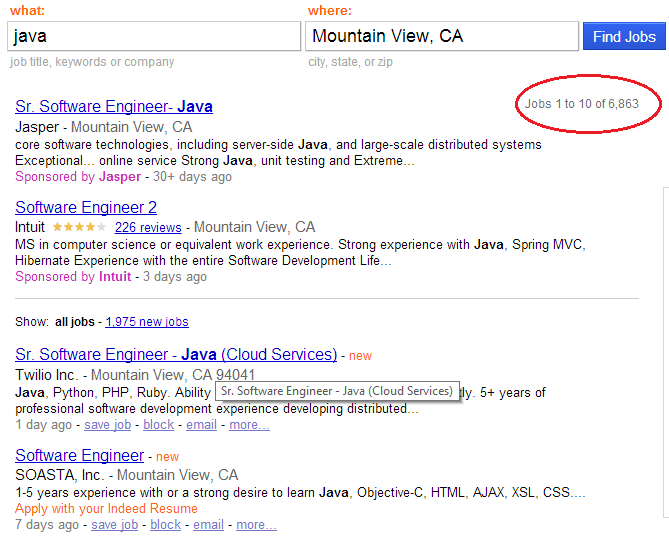
\includegraphics[scale=0.6]{images/indeed1.png}
  \caption{Search result of Indeed.com}
  \label{fig:Indeed}
\end{figure}

The reason for such a result is because current job searching web sites use the same information retrieval technology like ``Inverted index'' \cite{zobel2006inverted} as the common search engines, which just use keywords to map all the stored documents. Modern search engines all have some ranking algorithms to sort the search result, like page rank \cite{page1999pagerank}, so the top results always be the most related ones. But such algorithms are unavailable to the job search systems, because the criteria  of how to rank the job searching result is very personalized. A great job opening for one job seeker maybe looks not good to the other, because the goodness of a job to a specular job seeker is heavily depend on his personal background, like his education or professional experience etc.

Since the people's r\'esum\'es contain the most important background information, we believe the content of the r\'esum\'e could be used to rank the job openings. In this paper, we created a web system which uses the r\'esum\'es of job seekers to find the jobs that match their profiles best. The main idea is to calculate the similarity between the r\'esum\'e model and job models, which should be generated from r\'esum\'es and job descriptions. We want to transfer the job searching task from key word searching to candidate model matching. The matching result should be sorted by the matching score, higher matching score means a better matching. The matching algorithm does not only help job seekers to find the appropriate jobs, but also offers priority to them~\cite{gueutal2006brave}.  The job with higher matching score means the job is more appropriate to the job seeker, and if he applies to the job, the chance of getting the interview will be higher as well. Figure~\ref{fig:Matching} shows how this approach works.


\begin{figure}[htbp]
  \centering
  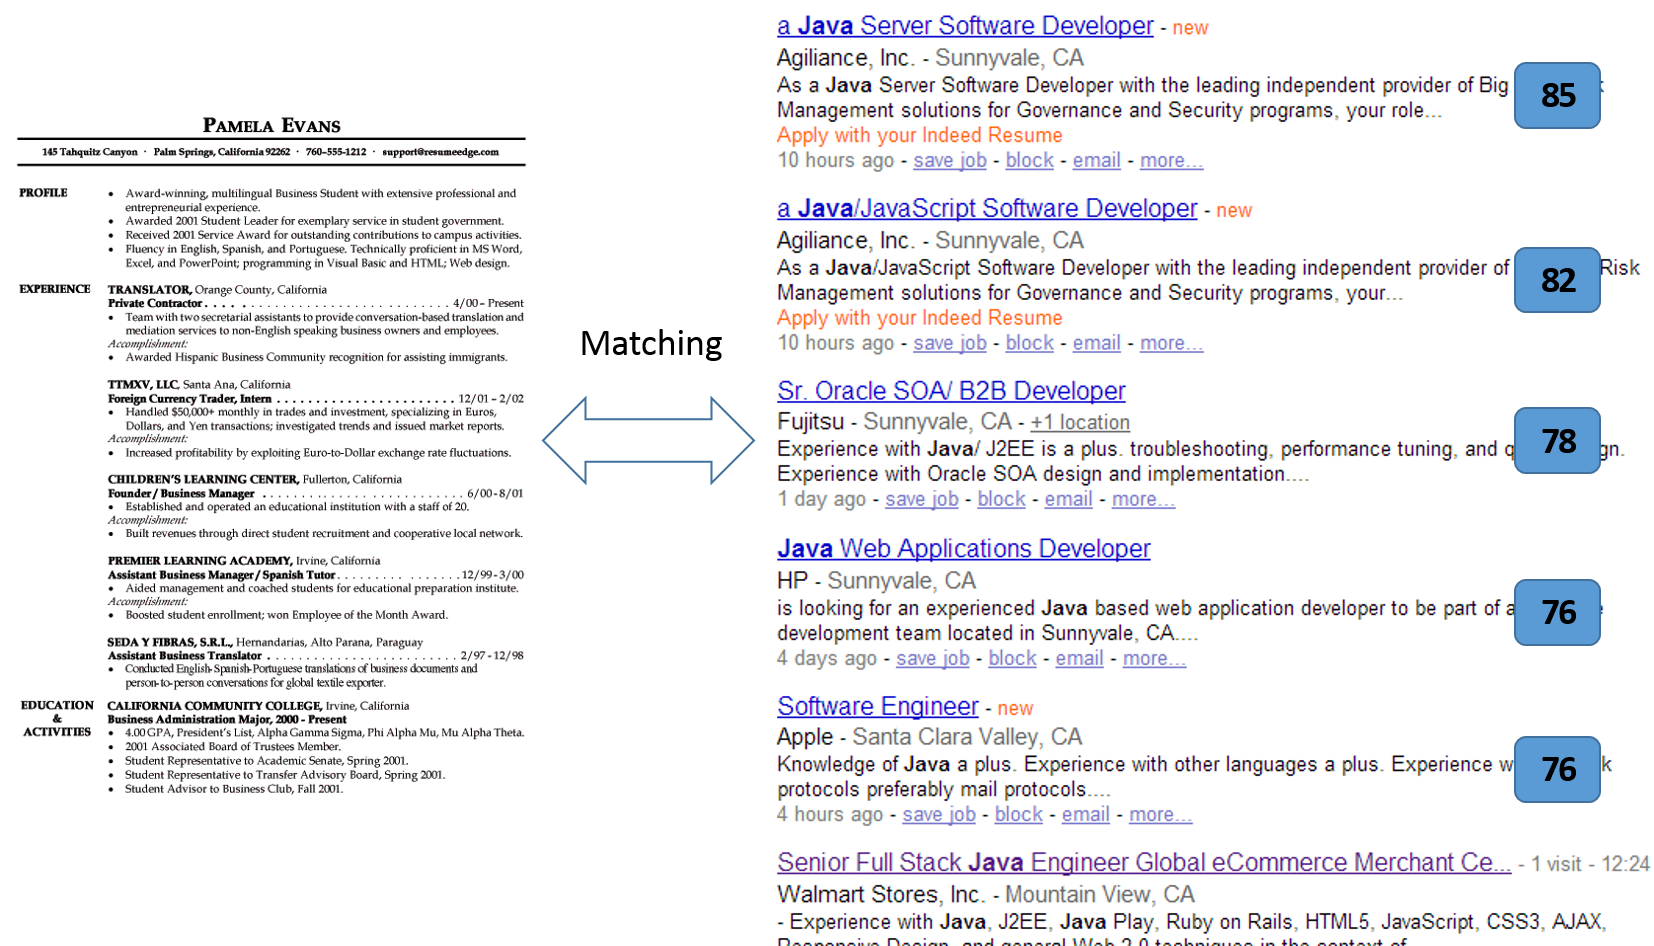
\includegraphics[scale=0.3]{images/matching.png}
  \caption{Matching the jobs with Resume}
  \label{fig:Matching}
\end{figure}

We make the following contributions in this work:

\begin{enumerate}
    \item  We proposed a r\'esum\'e - job matching system.
    \item  We proposed a finite state transducer based matching tool to extract information from unstructured data source, which is a lightweight and flexible library, and can be extended in very easy ways.
    \item  We proposed a semi-automatic approach, which can collect technical terms from hr data sources, and by which we created a domain specific ontology for recruitment.
    \item  We proposed statistical-based ontology similarity measure, which can measure the similarities between technical terms .
\end{enumerate}

The subsequent chapters are organized as follows: Section 2 describes what has been done in terms of prior work. Section 3 gives a overview of our system, R\'esuMatcher, the Personalized R\'esum\'e-Job Matching System. In section 4 and 5, we explains details of how we resolve the problems of information extraction and model similarity calculation. Section 6 describe the evaluation result of our system. Finally Section 7 shows the conclusions and future line of work. 